\documentclass[article]{sa}

%%%%%%%%%%%%%%%%%%%%%%%%%%%%%%
%% declarations for sa.cls %%%
%%%%%%%%%%%%%%%%%%%%%%%%%%%%%%
%%%%%%%%%%%%%%%%%%%%%%%%%%%%%%%%%%%%%%%%%%%%%%%%%%%%%%%%%%%%%%%
%% Based on the article latex template
%% of the Journal of Statistical Software
%% by Achim Zeileis
%% Reformated for SocArXiv by Chris Marcum <cmarcum@uci.edu> 
%%%%%%%%%%%%%%%%%%%%%%%%%%%%%%%%%%%%%%%%%%%%%%%%%%%%%%%%%%%%%%%


%% almost as usual
\author{Robert Z. Selden, Jr.\\Stephen F. Austin State University and Jean Monnet University}
\title{A Preliminary Study of Smithport Plain Bottle Morphology in the Southern Caddo Area}

%% for pretty printing and a nice hypersummary also set:
\Plainauthor{Robert Z. Selden, Jr.} %% comma-separated
\Plaintitle{A Preliminary Study of Smithport Plain Bottle Morphology in the Southern Caddo Area} %% without formatting
\Shorttitle{A Preliminary Study of Smithport Plain Bottle Morphology} %% a short title (if necessary)

%% an abstract and keywords
\Abstract{
This study expands upon a previous analysis of the Clarence H. Webb collection, which resulted in the identification of two discrete shapes used in the manufacture of the base and body of Smithport Plain bottles. The sample includes the Smithport Plain bottles from the Webb collection, and four new bottles: two previously repatriated specimens in the Pohler Collection, and two from the Mitchell site (41BW4) to test whether those specimens align morphologically with the Belcher Mound or Smithport Landing specimens. Results indicate significant allometry and a significant difference in Smithport Plain body and base shapes for bottles produced at the Smithport Landing and Belcher Mound sites in northwest Louisiana. The Pohler and Mitchell specimens do not differ significantly from those found at Smithport Landing or Belcher Mound. Analysis of the aggregated sample indicates some significant relationships between bottle shape and size, bottle shape and type, and bottle shape and site, highlighting assemblage-level and type-specific variability. The test of morphological disparity by period indicates a possible gradual trend toward standardization, and the test of morphological integration indicates that Caddo bottles are significantly integrated, meaning that those discrete traits used to characterize their shape (rim, neck, body, and base) vary in a coordinated manner. The iterative development of this research design can lead to substantive theoretical gains that augment and bolster discussions of Caddo ceramic morphological organization and vessel production.
}
\Keywords{American Southeast, Caddo, NAGPRA, 3D, geometric morphometrics, morphological disparity, morphological integration, virtual archaeology}
%% Publication information
%% Edit as needed depending on status of manuscript. 
%% Replace Preprint with journal short name of accepted
%% Pubs if copyright is open compliant. Add punctuation
%% for formatting as desired.
\Journal{Preprint}
\Volume{Vol. 89}
\Issue{} %Enter as "(Issue)" for APA
\Pages{} %Enter as "pp. m---n" for APA
\Year{2018}
\Submitdate{\today} %Enter date you submitted preprint for review
\Acceptdate{\today} %Enter date your paper was accepted for publication
\DOI{10.17605/OSF.IO/ESGXC}
%% The address of (at least) one author should be given
%% in the following format:
\Address{
  Robert Z. Selden, Jr.\\
  Center for Regional Heritage Research, Stephen F. Austin State University\\
  Cultural Heritage Department, Jean Monnet University\\
  E-mail: \email{zselden@sfasu.edu}\\
  URL: \url{https://hrc.sfasu.edu/}
}
%% It is also possible to add a telephone and fax number
%% before the e-mail in the following format:
%% Telephone: +43/512/507-7103
%% Fax: +43/512/507-2851

%% for those who use Sweave please include the following line (with % symbols):
%% need no \usepackage{Sweave.sty}

%% end of declarations %%%%%%%%%%%%%%%%%%%%%%%%%%%%%%%%%%%%%%%%%%%%%%%


\begin{document}

%% include your article here, just as usual
%% Note that you should use the \pkg{}, \proglang{} and \code{} commands.

\section*{}
Defined as ``a vessel with a spheroid or oval body, surmounted by a slender, cylindrical neck,'' Caddo bottles were initially seen as a somewhat homogenous ceramic form \cite[187]{RN2151}; some with shapes and motifs so similar to be deemed the work of a single maker \cite[188]{RN2151}. In a more recent study, Caddo bottles were found to be more symmetrical than bowls and ollas \citep{RN11521}; however, additional work is needed to identify whether—and to what extent—this holds true across a broader range of vessel shapes and types. Caddo vessel shapes are variable among groups and through time, reflecting stylistic, functional, and social change \citep{RN1986}. Caddo potters elevated local ceramic production to high art, and ``had no superiors short of the Pueblo country'' \citep[239]{RN491}, leading some analysts to posit that Caddo bottles rest at the apex of Native American ceramic technology \citep{RN1867}. A division of the Caddo bottle category has been proposed for northeast Texas that segregates bottle forms into 27 shapes, each with distinct temporal and spatial distributions \citep[Figure 2]{RN11636}, and novel deployments of geographic information systems are aiding in the refinement of their probable geographic extents \cite{RN2674}.

This effort capitalizes on the quiddity of Caddo bottle shape for a small sample (n = 8) of Smithport Plain bottles previously posited to exhibit morphological differences \citep{RN11716,RN870,RN5266}. Three-dimensional (3D) meshes for the Webb Collection and four new samples from one site and one collection were used to test whether a significant difference in shape exists for Smithport Plain bottles by site, followed by a test for allometry. The Smithport Plain bottles were subsequently examined as part of the aggregated sample of Caddo bottles to demonstrate morphological variability, allometry, morphological disparity, and morphological integration among the types (Table 1 and Figure ~\ref{fig:fig1}).

\begin{figure}[ht]\centering
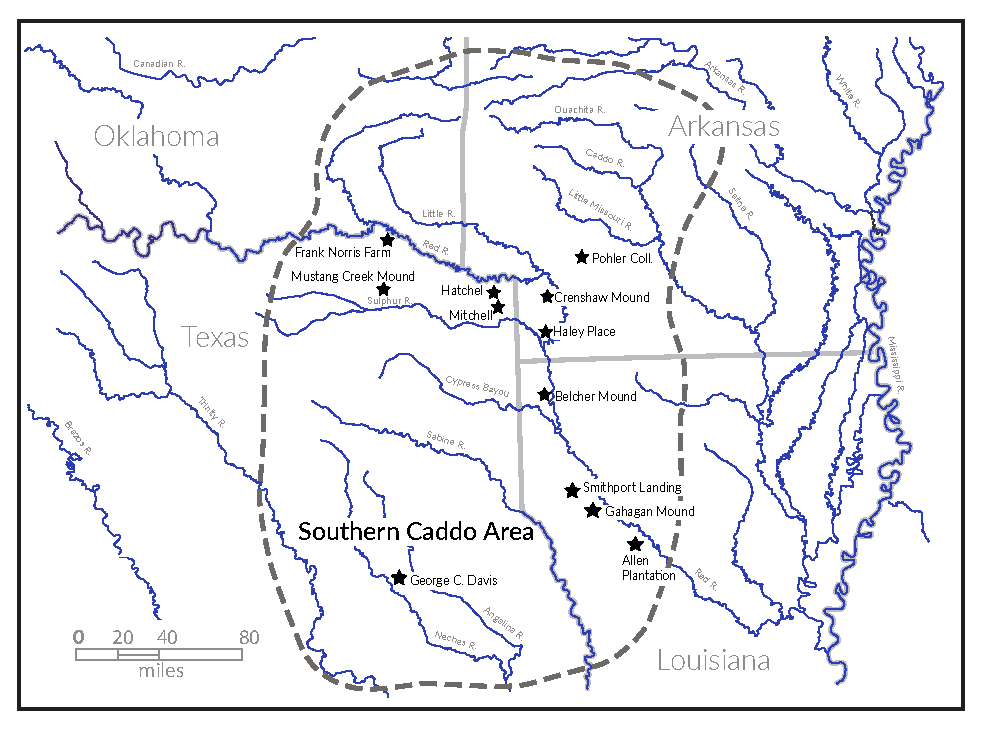
\includegraphics[width=\linewidth]{Figure_01}
\caption{Locations of Allen Plantation, Hatchel, Belcher Mound, Crenshaw Mound, Frank Norris Farm, Gahagan Mound, George C. Davis, Haley Place, Mustang Creek Mound (also known as T. N. Cole), Paul Mitchell (Mitchell), specimens from the Pohler Collection (Clark County, Arkansas), and Smithport Landing.}
\label{fig:fig1}
\end{figure}

Taxonomic definitions for Caddo ceramics integrate semiotic and morphological attributes, and each type is characterized by a broad range of vessel shapes that often include bottles, bowls, carinated bowls, ollas, as well as other shapes \citep{RN870,RN5066}. The Smithport Plain type was defined by Clarence H. Webb \citep{RN5266} at the Smithport Landing site (16DS4) in northwest Louisiana and is believed to range in age from the Formative to Early Caddo periods (AD 800 - 1200) \citep{RN5270}. All Caddo bottles used in this analysis fall under the Native American Graves Protection and Repatriation Act (NAGPRA), excepting those found in House 6 at the Belcher Mound site (Table 1). The Caddo Nation of Oklahoma granted permission to scan the collections with the provision that any scan data used in the analysis must not include the texture (color) file. Full-resolution scan data were forwarded to the Caddo Nation of Oklahoma with the texture applied. This provides them with an accurate 3D record of each vessel, and a means of viewing a collection of bottles that is curated across numerous repositories.

\subsection*{Geometric morphometrics in archaeology}

Analyses of artifact shape are neither new or novel \citep{RN11779}, thus it is not surprising that geometric morphometrics (GM) (sensu Marco Corti \citep{RN11559}) has captivated analysts of material culture due to the substantive contribution of morphology to lithic \citep{RN11529,RN369,RN11534} and ceramic typologies \citep{RN1752,RN11631,RN305}, additional categories of material culture \citep{RN1737,RN4374,RN11527}, and novel applications \citep{RN11543,RN11544}. The earliest study in archeology was an analysis of irregular shapes by elliptic Fourier analysis (EFA) \citep{RN4379}, and the adoption of the method by the archaeological community has grown to include an impressive array of applications (Figure ~\ref{fig:network}).

\begin{figure}[ht]\centering
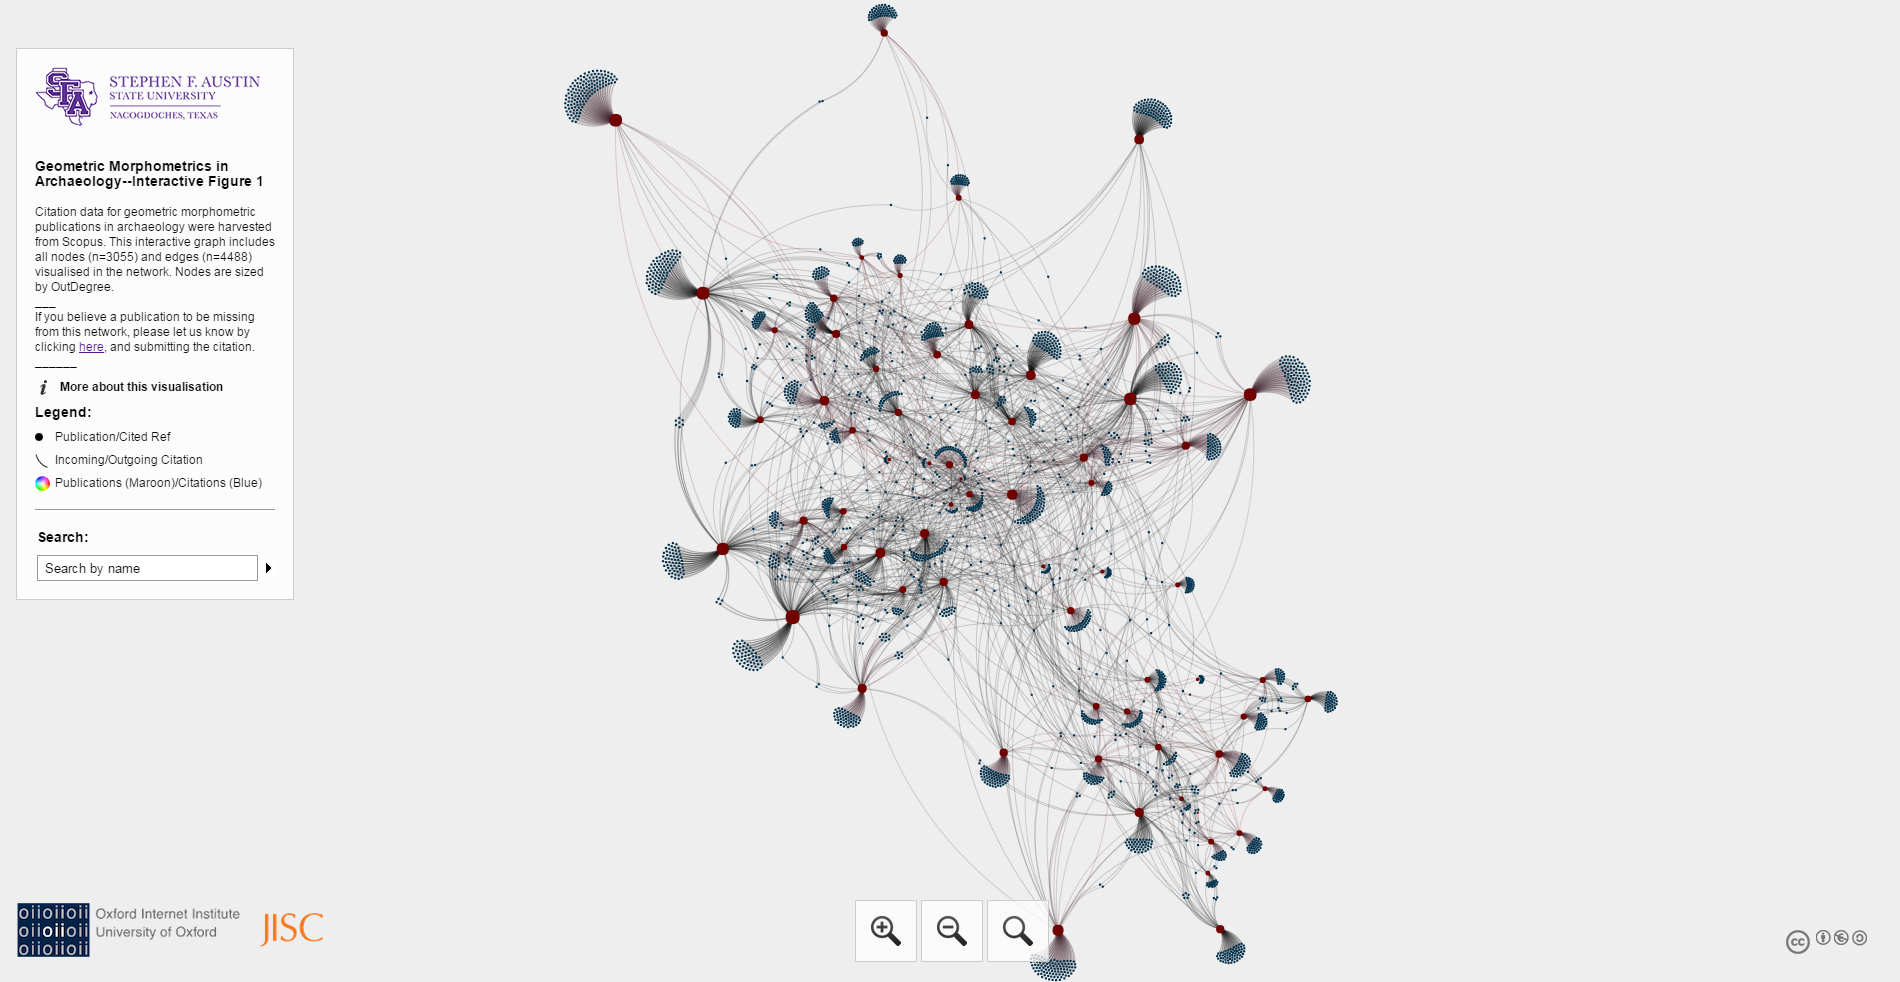
\includegraphics[width=\linewidth]{Figure_02}
\caption{Interactive citation network for geometric morphometric studies in archaeology \href{http://crhr-archive.sfasu.edu/GMArchFig1/}{http://crhr-archive.sfasu.edu/GMArchFig1/}.}
\label{fig:network}
\end{figure}

EFA has been employed at an increasing rate in lithic and ceramic analyses \citep{RN4394,RN4327,RN11529,RN4350,RN4373,RN4338,RN4353,RN11627,RN305}, where new approaches continue to be developed that advance archeological applications. Creative research designs are also being developed to address challenges with incomplete specimens in the archeological record \citep{RN11575,RN11574,RN11539,RN11533,RN11730}. These advancements have aided in the development of a useful suite of protocols applicable to wide-ranging research questions.

The recent fluorescence of landmark-based applications has been driven by advances in anthropology \citep{RN11531,RN1770,RN306,RN1732} and a variety of other research domains \citep{RN11558,RN1743,RN1762,RN4775,RN11553,RN11535,RN11526,RN11557,RN11554,RN1646,RN11541,RN478,RN11560} that articulate with the rise of the Procrustes paradigm \citep{RN1743}. Archaeological applications have included two-dimensional (2D) analyses of Clovis technology in North America \citep{RN1754,RN1736,RN11628,RN4378,RN11625}, Fishtail or Fell projectile points in South America \citep{RN4346,RN11545}, bifacial points from the Umbu Tradition in Brazil \citep{RN11547,RN370,RN11548}, lanceolate points—ayampitin—from Argentina \citep{RN11549}, the size and shape of projectile points from southern Patagonia \citep{RN4344,RN4345}, bifacial tools from southern Poland \citep{RN11551}, Final Palaeolithic large tanged points \citep{RN4738}, Paleoindian point types from Florida \citep{RN369} and the Southern High Plains \citep{RN4358}, ceramics from Casas Grandes \citep{RN11631}, flake morphology \citep{RN4334}, and reduction effects \citep{RN4349}; all of which capitalize on the morphological variation that occurs in a single plane \citep{RN1754,RN11542}.

For research designs that incorporate questions associated with more complex geometry, 3D landmark-based approaches may be more appropriate. Examples from the literature include the development of novel tools and applications \citep{RN1722} that cover a broad range of artifact categories including projectile points \citep{RN1750,RN1755}, bifaces \citep{RN1727,RN4392,RN11550}, percussive tools \citep{RN1772}, flake scars \citep{RN4337}, flake tools \citep{RN11552}, handaxes \citep{RN1730,RN1766,RN1733,RN3145,RN335}, and Caddo ceramics \citep{RN11521,RN11716,RN1994}. This study adduces the variation that occurs within a single plane (widest vessel profile) for a sample of Caddo bottles; however, 3D data were required to identify the widest profile. Additionally, a variety of landmark and semilandmark configurations are in development that provide for a more robust analysis of 3D morphology associated with specific elements of vessel morphology.

\section*{Methods}

Bottles were scanned with a Creaform GoSCAN 50 at a 0.8 mm resolution or a Creaform GoSCAN20 at 0.5 mm resolution depending on their size. Scanner calibration was optimized prior to each scan, with positioning targets required for increased accuracy, and shutter speed reconfigured in each instance. A clipping plane was established to reduce the amount of superfluous data collected during each scan. Following data collection, resolution for the GoSCAN 50 meshes was increased to 0.5 mm, and meshes from both scanners were transferred to VXmodel where the final mesh was rendered following application of the clean mesh function. This was used to remove isolated patches, self-intersections, spikes, small holes, singular vertices, creased edges, narrow triangles, outcropping triangles, narrow bridges, and non-manifold triangles prior to export as an ASCII stl file. The stl functions as a backup, and the ply was subsequently imported to Geomagic Design X (Dx).

Prior to pursuing the mixed-method analysis employing data from two different scanners, two meshes of the same object---produced with the Creaform GoSCAN 50 and GoSCAN 20---were imported to a computer-aided inspection program (Geomagic Control X) in an effort to identify any significant deviations that may exist between the meshes prior to the GM analysis (Figure ~\ref{fig:fig3}). The tolerance level for the inspection was selected by using the highest resolution of the GoSCAN 20 (0.1 mm). Small areas of the rim exhibited minor differences while the remainder of the vessel is within the arbitrary 0.1 mm tolerance; thus, results fell within an acceptable error range.

\begin{figure}[htbp]\centering
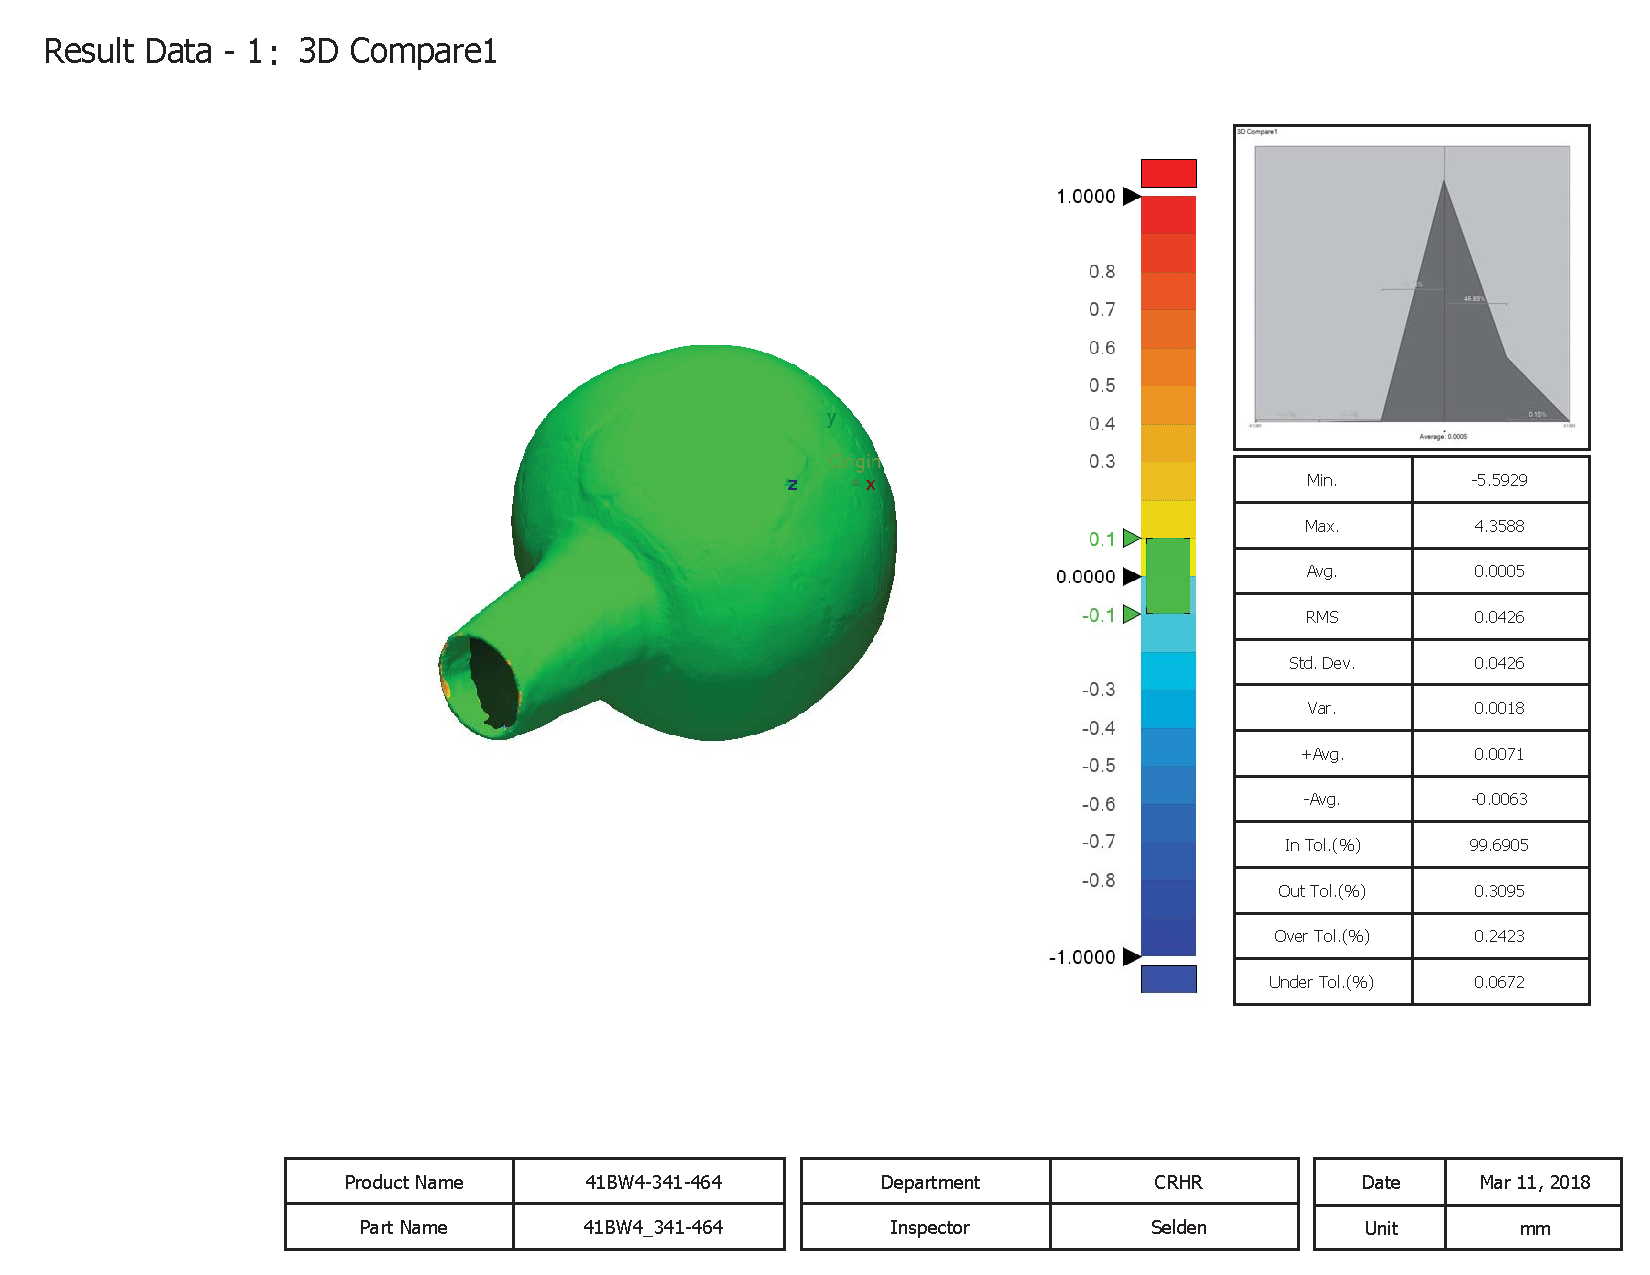
\includegraphics[width=\linewidth]{Figure_03}
\caption{Results of 3D compare for the GoSCAN 50 and GoSCAN 20 meshes of bottle 41BW4 341-464 indicating that 99.6905 percent of the vessel falls within the arbitrary 0.1 mm tolerance.}
\label{fig:fig3}
\end{figure}

The histogram shown in Figure ~\ref{fig:fig3} illustrates the Gaussian distribution for the number of errors over the whole deviation. The graph is split into six segments: 1-Sigma at 31 percent from the average to the maximum deviation in each direction, 2-Sigma at 69 percent from the average to the maximum deviation in each direction, and 3-Sigma at 93.3 percent from the average to the maximum deviation in each direction. The average (AVG) is the sum of all deviations divided by the number of all deviations, and the RMS is the square root of all squared deviations divided by the number of all deviations (sometimes referred to as the effective deviation). In tolerance (In Tol) and out tolerance (Out Tol) percentages indicate the percentage of deviations in or out of a given tolerance, and over tolerance (Over Tol) and under tolerance (Under Tol) percentages indicate the percentage of deviations over (positive direction) or under (negative direction) the tolerance range by the mesh normal of the reference mesh.

\subsection*{Alignment and reference geometry}

Following transfer to Dx, each mesh was subjected to an additional quality check to eliminate non-manifold poly-vertices, folded poly-faces, dangling poly-faces, small clusters, small poly-faces, non-manifold poly-faces, crossing poly-faces, and small tunnels. Due to the paucity of homologous landmarks on cultural artifacts \citep{RN1730}, reference geometry was constructed around each vessel in a manner that yielded a replicable configuration of nine landmarks, and 46 equidistant semilandmarks along the widest vessel profile, with notable similarities to previous landmark configurations used by \cite{RN1752}, \cite{RN1994}, and \cite{RN11631}, all of which largely follow \cite{RN11755}.

The first component of reference geometry added, and the principal assumption, was a reference vector. A sampling ratio of 100 percent was used to apply the reference vector on a revolving axis, after which a reference point was added by projecting it atop the mesh surface at the location where the reference vector exits the base of the vessel. A reference plane was inserted using the pick multiple points function, by adding a series of 10 points around the circumference of the bottle's base. Each element of reference geometry (vector, point, and plane) was then used in an interactive 3-2-1 alignment where the vessel was aligned to a global origin, orienting it in 3D space where it sat upright atop a planar surface (assumed to be the intent of the maker). Following alignment, the reference plane and point were deleted.

The widest profile is defined as the location on a mesh that lies farthest from that point where the reference vector exits the vessel base while oriented atop the planar surface. To identify that location, a mesh sketch was generated with the planar method using the plane at the base of the vessel to identify and sketch the widest vessel circumference. By using the plane located at the base of the vessel for the sketch, the point at which the reference vector exits the mesh remains linked to the remainder of the reference geometry. A circle was then sketched using the vector as the center, extending outward until the whole of the vessel fits within. Using the mesh sketch, a cylinder (surface) was extruded around the vessel. The accuracy analyzer in Dx was then used to identify the point on the vessel with the lowest deviation from the extruded surface, and a plane (MPlane) was inserted coplanar to the vector and oriented to the widest point, bisecting the vessel along the widest profile.

Using the MPlane as the basis for a second mesh sketch, a spline with 15 interpolation points was sketched on one rim. Above that sketch, a horizontal line was added where both the spline and horizontal line were used to determine the horizontal tangent of the rim. A vertical line was subsequently added that bisected the rim at the location of the tangent. This operation was repeated for the opposing rim. The addition of this added step was necessary because surface scanners are unable to collect data from the interior of the bottles, so the spline needed to be cut in a replicable location. Since the Smithport Plain bottles exhibit slightly inverted-to-vertical rims, the preceding step was extended to include an additional measure. A line was drawn between each rim tangent, then a second from the intersection of the line and reference vector to a point 10 mm down the vector, where a horizontal line (parallel with the rim peaks) was inserted to intersect with both external walls of the bottle. It is at this intersection that the final mesh sketch was cut to discriminate between the neck and rim. While this step admittedly appears odd in the context of a comparison of bottle shapes that all exhibit direct rims, it is of considerable import for inter-type comparisons where other bottle types exhibit differing rim morphologies (i.e., everted, etc.).

Using the MPlane as the basis for a third sketch, a spline was populated for the entirety of the silhouetted profile. That spline was split at the location of the horizontal tangent on each rim, and the remaining sections that continued into the bottle interior were deleted. The second split was added at the intersection of the spline and reference vector (center of base). Four additional splits were subsequently added at the juncture of the base/body and body/neck on each side of the vessel at the points of highest curvature. The point of highest curvature used to split the spline was identified using the curvature function in Dx, and does not represent an arbitrary location.

\subsection*{Landmarks and semilandmarks}

A total of nine landmarks and 46 semilandmarks segregated each bottle into four discrete components corresponding with the rim, neck, body, and base (Table 2 and Figure ~\ref{fig:fig4}). Landmarks and semilandmarks were populated along the spline, and numbering always began on that side of the profile determined to include the widest point. Divisions between each component articulate with those of the spline splits, where landmarks were placed at each of the points in Table 2, with a series of equidistant semilandmarks between them.

\begin{figure}[ht]\centering
\includegraphics[width=\linewidth]{Figure_04}
\caption{Spline splits for discrete components (rim, neck, body, and base) used in the GM analysis (left) segregated by landmarks (blue), with equidistant semilandmarks (white) populated between (right).}
\label{fig:fig4}
\end{figure}

While sliding semilandmarks were an early consideration of this research design, the decision to use equidistant semilandmarks rather than sliding semilandmarks is based upon results from an earlier iteration of the Webb collection analysis \citep{RN11716}. In the study of the Webb collection, the first landmark and sliding semilandmark configuration did not split the spline between the neck and rim, and when mean shapes were generated for each type, an anomaly, from the everted rims of Belcher Engraved bottles in that case, was added to the otherwise direct or tapered necks of the Hickory Engraved and Smithport Plain bottles. Given that the use of sliding semilandmarks could potentially influence the results of this analysis by introducing a morphological attribute to specimens where one does not exist, they were abandoned.

\subsection*{Analysis}

Landmarks and equidistant semilandmarks were exported as x, y, and z coordinate data from Dx. Those data were aligned to a global coordinate system \citep{RN11622,RN11623,RN11563}, achieved through generalized Procrustes superimposition \citep{RN478} performed in R 3.5.0 \citep{RN477} using the geomorph library v.3.0.6 \citep{RN11530,RN1774}. Procrustes superimposition translates, scales, and rotates the coordinate data to allow for comparisons among objects \citep{RN11564,RN478}. The geomorph package uses a partial Procrustes superimposition that projects the aligned specimens into tangent space subsequent to alignment in preparation for the use of multivariate methods that assume linear space \citep{RN1646,RN11563}.

Principal components analysis \citep{RN1746} was used as an exploratory means of visualizing shape variation among the bottles. The shape changes described by each principal axis are commonly visualized using thin-plate spline warping of a reference 3D mesh \citep{RN1731,RN479}. A residual randomization permutation procedure (RRPP; n=1000 permutations) was used for all Procrustes ANOVAs \citep{RN1655,RN11775}, which has higher statistical power and a greater ability to identify patterns in the data should they be present \citep{RN1719}. To assess whether shape differs by size (allometry) and site, Procrustes ANOVAs \citep{RN1749} were run that also enlist effect-sizes (z-scores) computed as standard deviates of the generated sampling distributions \citep{RN1756}. For the aggregated sample, a Procrustes ANOVA was run to assess whether shape changes with size, and the assumption of allometric slope homogeneity was tested with the procD.allometry function using the PredLine option \citep{RN1649}. Should this test not be significant, then allometric slopes are similar---if not identical---across time and types.

A Procrustes ANOVA and pairwise test was used to identify sites where bottle shapes and types differ. The pairwise test is conceptually similar to trajectory analysis \citep{RN11573,RN1648,RN4445,RN1739} in that pairwise statistics are vector lengths between vectors, but differs in that a factorial model is not explicitly needed to contrast vectors between point factor levels nested within group factor levels \citep{RN11530}. Procrustes variance was used to discriminate between groups and to compare the amount of shape variation (morphological disparity) across communities \citep{RN11560}, which is estimated as the Procrustes variance using residuals of linear model fit \citep{RN11530}.

Morphological integration was assessed for the aggregated sample of whole vessels. Integration between pairs of traits was tested using a two-block partial least-squares (2B-PLS) analysis to evaluate relationships for two blocks of variables collected from the same specimens \citep{RN11615,RN11613,RN11614}, using shape coordinates in all blocks of variables \cite{RN11616,RN11615,RN11617}. To assess whether the different modules (RIM\textsubscript{neck}, NECK\textsubscript{body}, and BODY\textsubscript{base} in particular) are integrated, a two-sample test using effect sizes calculated as standard deviates in sampling distributions from the 2B-PLS analyses were used to determine the significance and strength of integration between the modules \citep{RN11700}.

\section*{Results}

The mean consensus configuration and Procrustes residuals were calculated using a generalized Procrustes analysis (GPA) (Figure ~\ref{fig:fig5}). This initial view of the data demonstrates the degree of variability in Caddo bottles that occurs across the sample. As an exploratory measure, GM methods—to include GPA—aid in clarifying shape differences, and in the production of novel a posteriori hypotheses \citep{RN1720}.

\begin{figure}[ht]\centering
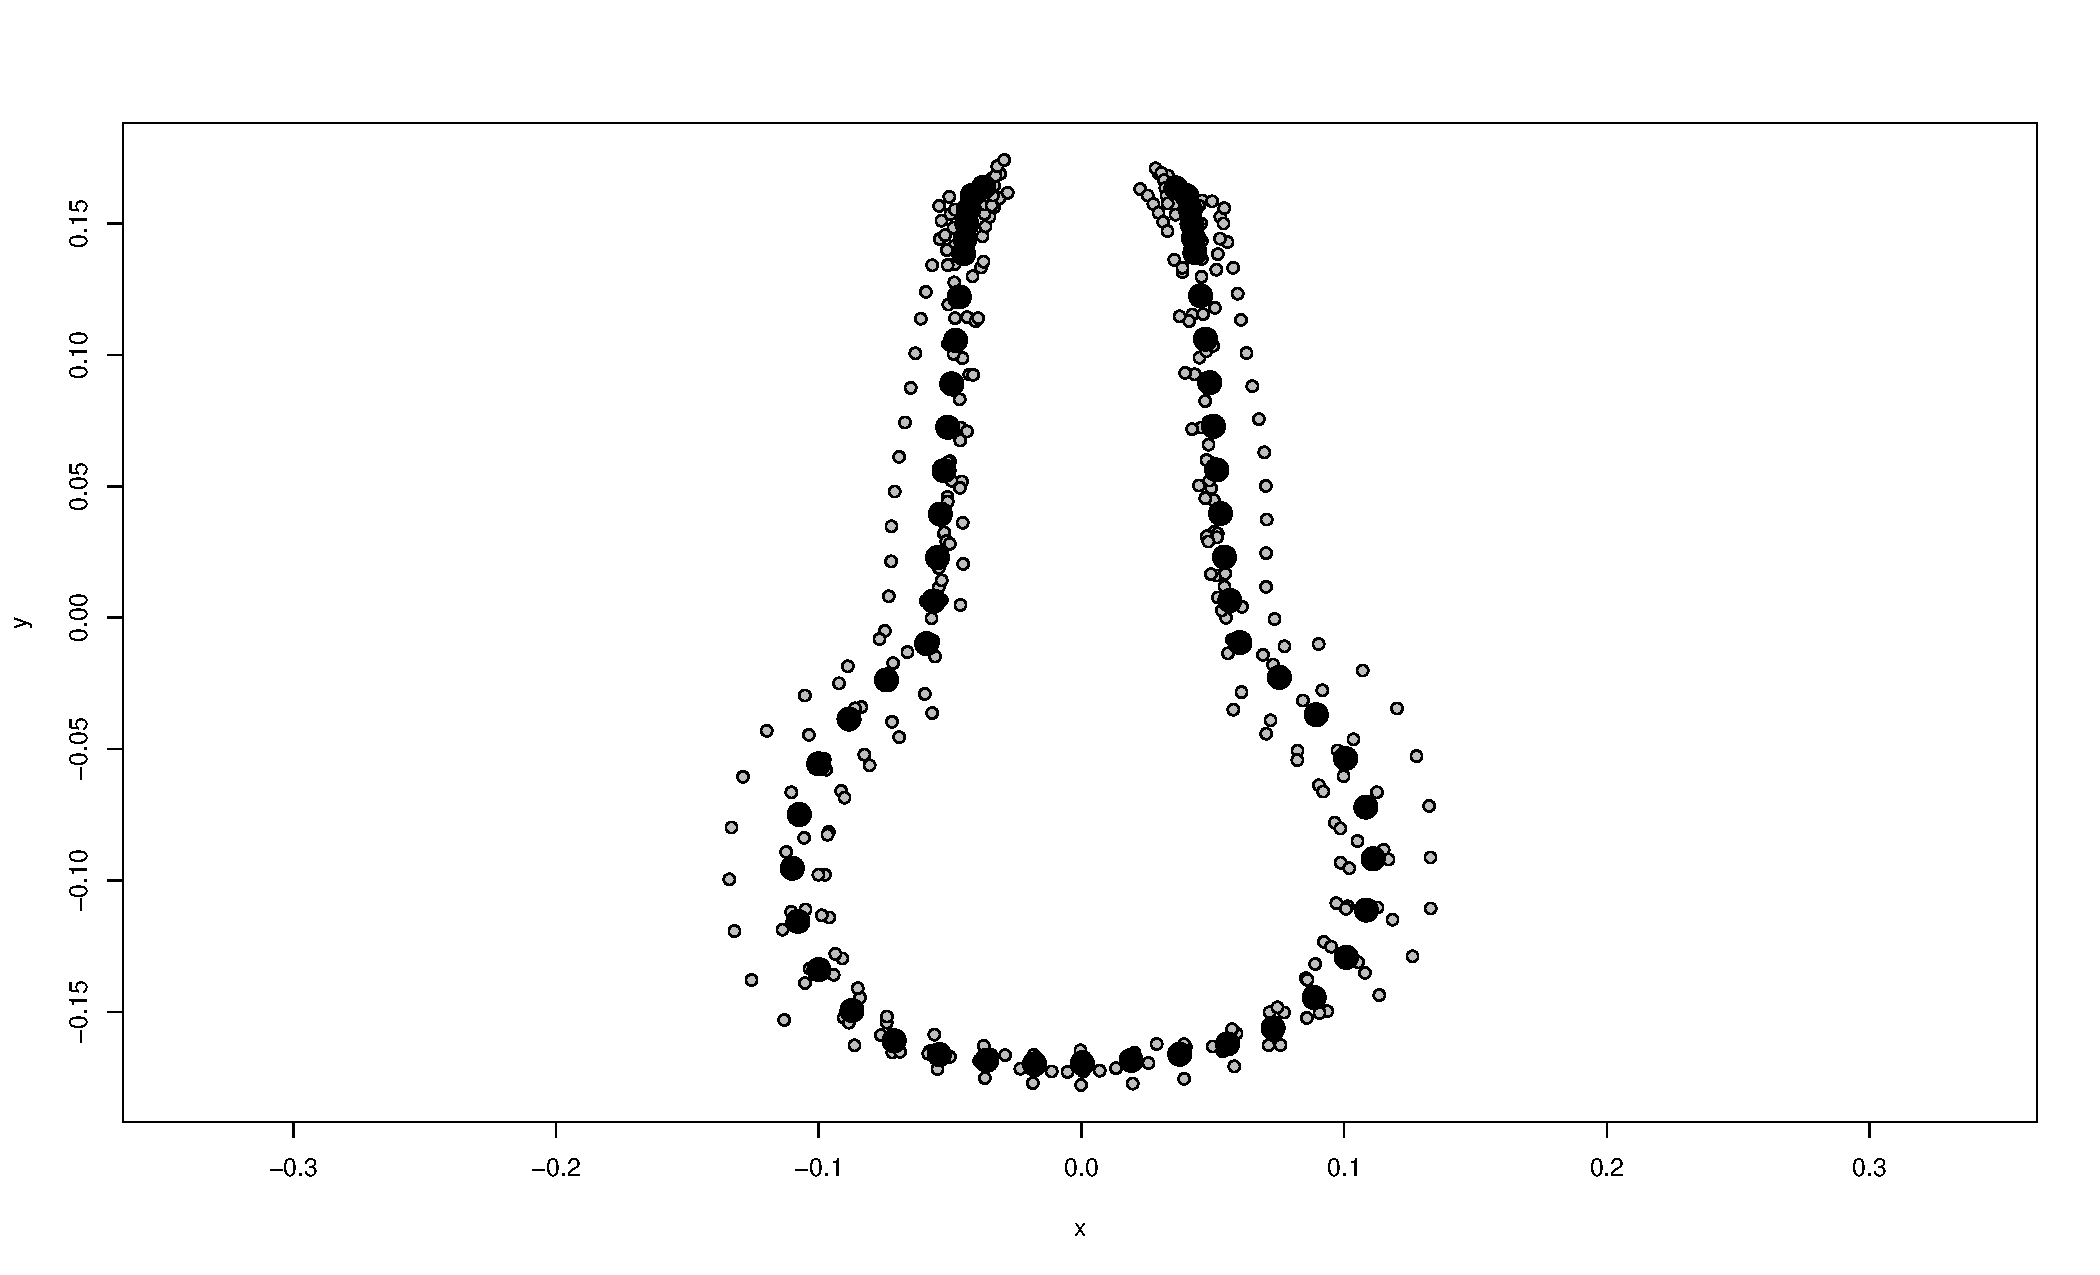
\includegraphics[width=\linewidth]{Figure_05}
\caption{Results of generalized Procrustes analysis for Smithport Plain whole bottles. Mean consensus configuration shown in black; samples in gray.}
\label{fig:fig5}
\end{figure}

Principal components analysis (PCA) was conducted on scaled, translated, and rotated landmarks and semilandmarks, and demonstrates that the first two PC’s account for 68 (PC1) and 27 (PC2) percent of the variation in bottle shape (Table 3 and Figure ~\ref{fig:fig6}). Together, PC1 and PC2 account for 95 percent of shape variation, with all remaining PCs representing three or fewer percent of the variation (Table 3). The first two PCs are plotted in Figure 6, where warp grids represent the shape changes along PC1 and PC2. This plot indicates that shape changes associated with PC1 articulate most readily with base and body shape, and shape changes associated with PC2 articulate with base, body, and neck shape.

\begin{figure}[ht]\centering
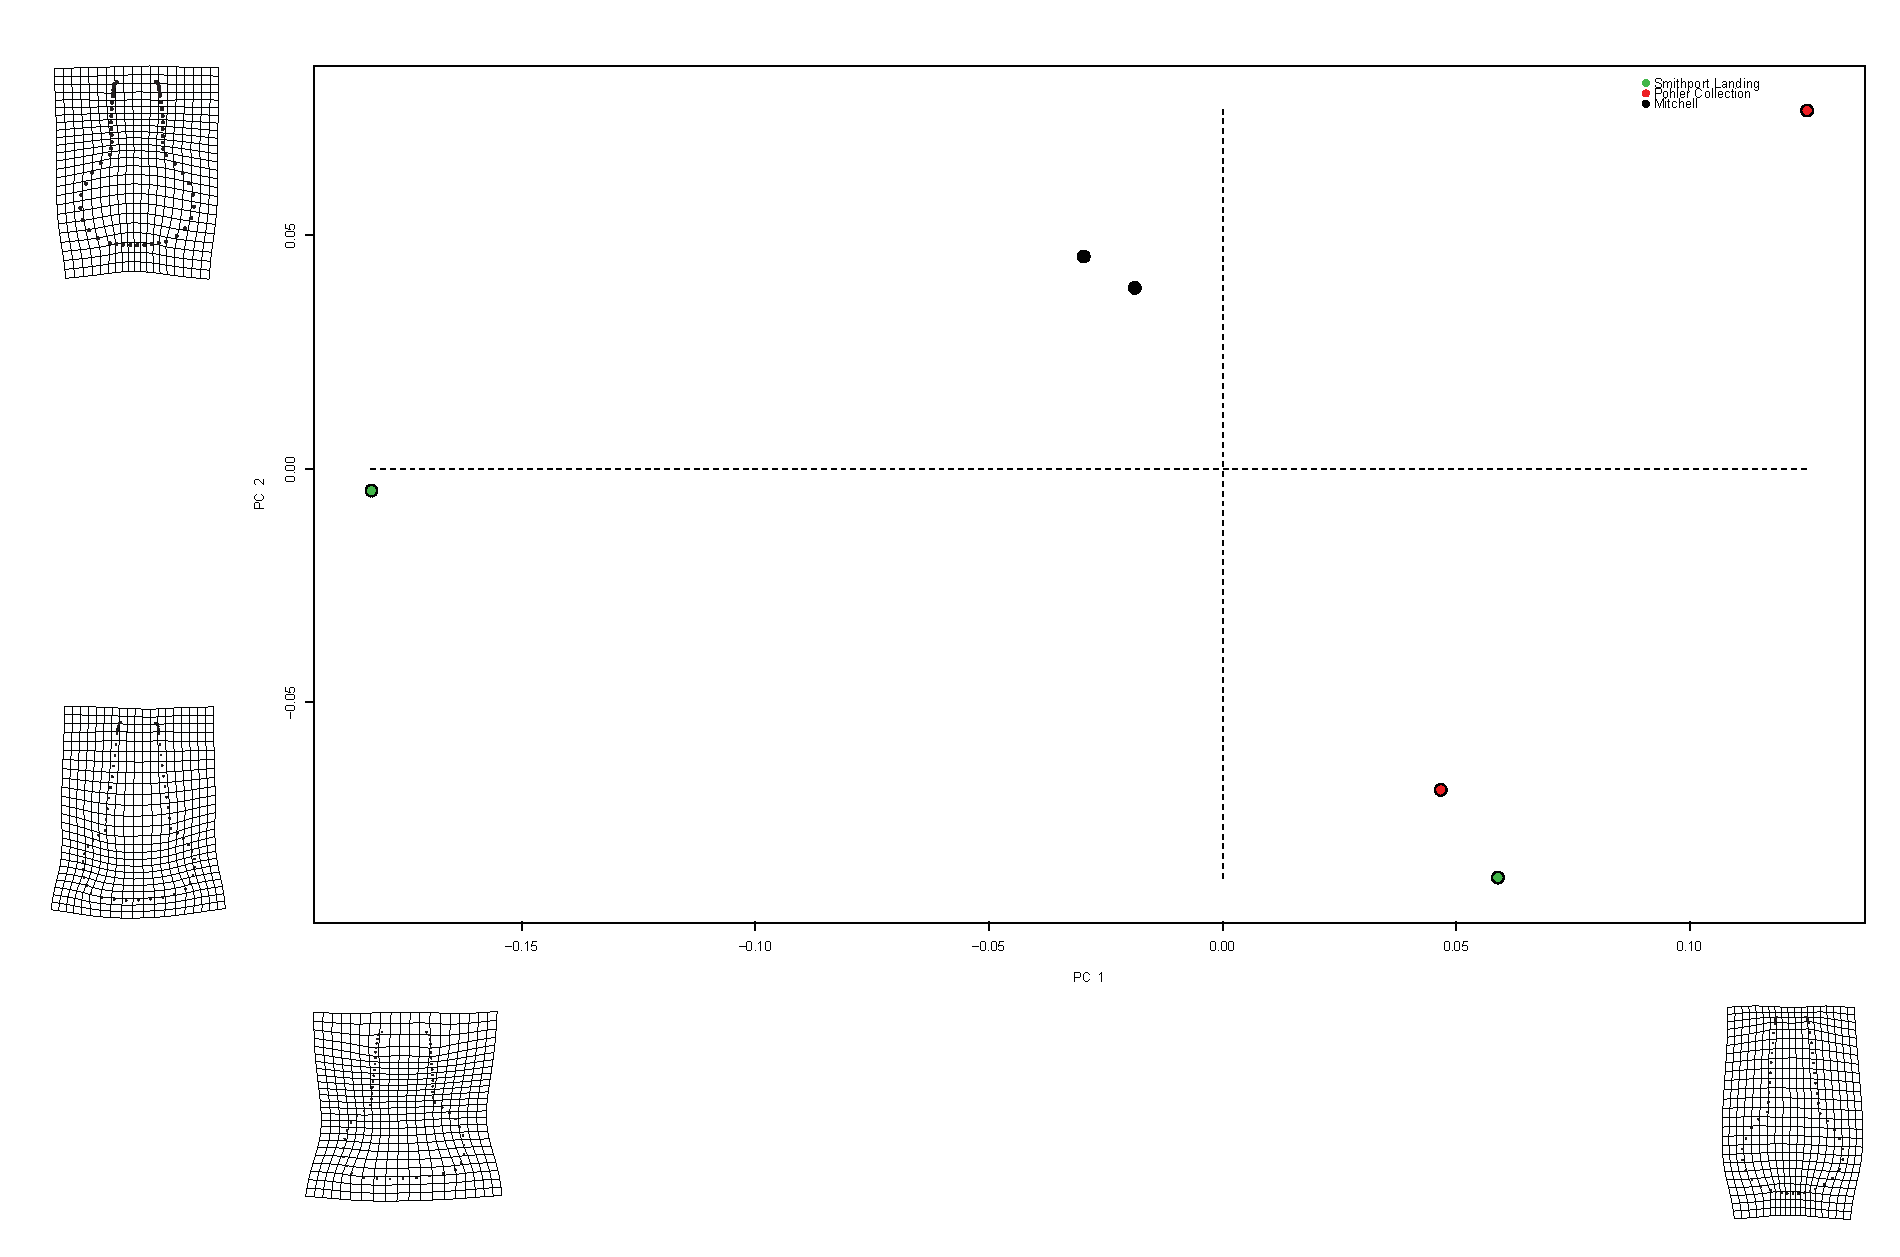
\includegraphics[width=\linewidth]{Figure_06}
\caption{Results of PCA summarizing shape variation in the whole bottle sample.}
\label{fig:fig6}
\end{figure}

A Procrustes ANOVA was used to test for significant allometry. Results of the ANOVA indicate significant allometry in the sample (RRPP = 1000, Rsq = 0.59427, Pr(>F) = 0.0075), indicating that Smithport Plain bottle shapes change with size. A Procrustes ANOVA was used to test for a significant difference in bottle shape by site, and results indicate that there is not a significant difference in bottle shape by site (RRPP = 1000, Rsq = 0.40907, Pr(>F) = 0.537).


%% Note: If there is markup in \(sub)section, then it has to be escape as above.
\bibliography{sa}

\end{document}
